\usetikzlibrary{fit,positioning, backgrounds}

\begin{adjustbox}{max width=\linewidth, max height=\textheight, keepaspectratio}
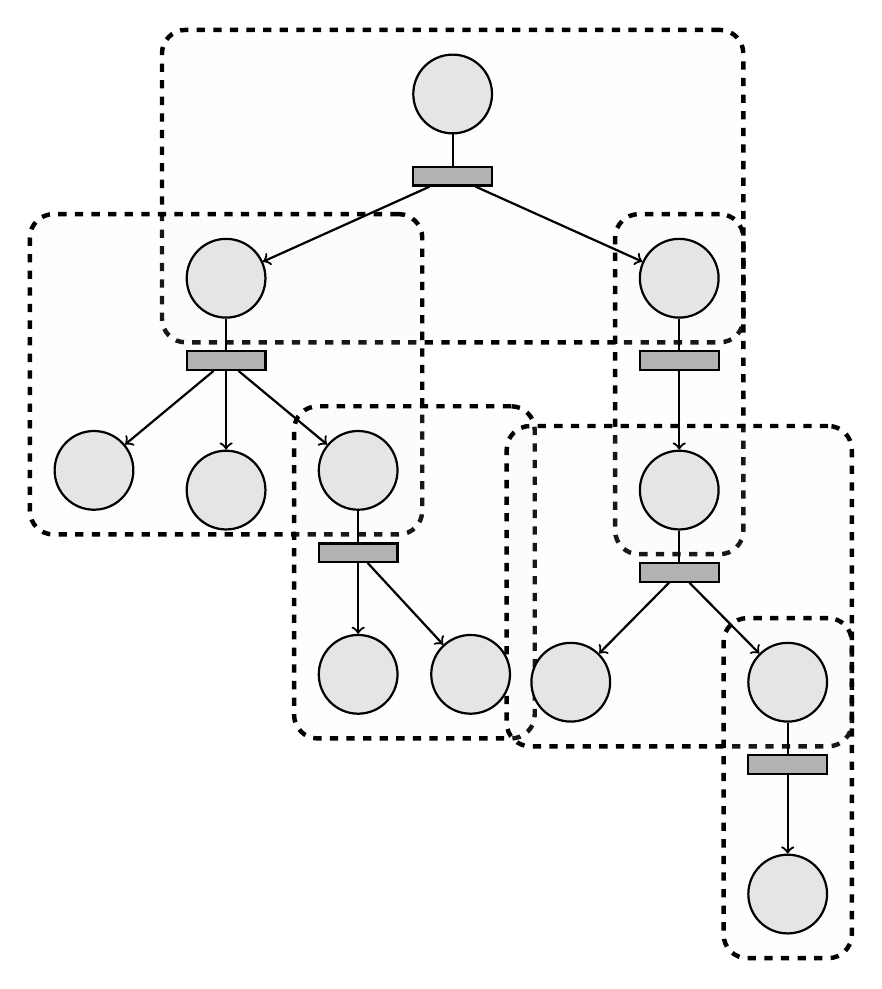
\begin{tikzpicture}[
    cNode/.style={circle, draw, minimum size=10mm, fill=black!10, thick, font=\small},
    sNode/.style={rectangle, draw, minimum width=10mm, minimum height=2mm, fill=black!30, thick},
    edge/.style={draw, thick},
    fStyle/.style={draw=black, ultra thick, dashed, fill=blue!5, fill opacity=0.1, rounded corners=3mm, inner sep=3mm}
]
    \node[cNode] (R) {};
    \node[sNode, below=0.4cm of R] (S) {};
    \path[edge] (R) -- (S);
    \node[cNode, below left=0.8cm and 2.0cm of S] (C1) {};
    \node[cNode, below right=0.8cm and 2.0cm of S] (C2) {};
    \path[edge] (S) edge[->] (C1) edge[->] (C2);
    \node[sNode, below=0.4cm of C1] (S1) {};
    \node[cNode, below left=0.9cm and 0.8cm of S1] (G1) {};
    \node[cNode, below=1.0cm of S1] (G2) {};
    \node[cNode, below right=0.9cm and 0.8cm of S1] (G3) {};
    \path[edge] (C1) -- (S1) (S1) edge[->] (G1) edge[->] (G2) edge[->] (G3);
    \node[sNode, below=0.4cm of G3] (S3) {};
    \node[cNode, below=0.9cm of S3] (GG1) {};
    \node[cNode, right=0.4cm of GG1] (GG2) {};
    \path[edge] (G3) -- (S3) (S3) edge[->] (GG1) edge[->] (GG2);
    \node[sNode, below=0.4cm of C2] (S2) {};
    \node[cNode, below=1.0cm of S2] (G4) {};
    \path[edge] (C2) -- (S2) (S2) edge[->] (G4);
    \node[sNode, below=0.4cm of G4] (S4) {};
    \node[cNode, below left=0.9cm and 0.5cm of S4] (GG3) {};
    \node[cNode, below right=0.9cm and 0.5cm of S4] (GG4) {};
    \path[edge] (G4) -- (S4) (S4) edge[->] (GG3) edge[->] (GG4);
    \node[sNode, below=0.4cm of GG4] (S5) {};
    \node[cNode, below=1.0cm of S5] (GGG1) {};
    \path[edge] (GG4) -- (S5) (S5) edge[->] (GGG1);

    \begin{scope}[on background layer]
    \node[fStyle, fit=(R) (S) (C1) (C2)] (F0) {};
    \node[fStyle, fit=(C1) (S1) (G1) (G3)] (F1) {};
    \node[fStyle, fit=(C2) (S2) (G4)] (F2) {};
    \node[fStyle, fit=(G3) (S3) (GG1) (GG2)] (F3) {};
    \node[fStyle, fit=(G4) (S4) (GG3) (GG4)] (F4) {};
    \node[fStyle, fit=(GG4) (S5) (GGG1)] (F5) {};
    \end{scope}
\end{tikzpicture}
\end{adjustbox}
